\documentclass[a4paper,10pt]{report}
\usepackage{cours}
\newcommand{\Sum}[2]{\ensuremath{\textstyle{\sum\limits_{#1}^{#2}}}}

\begin{document}
\everymath{\displaystyle}


\begin{center}
 \shadowbox{{\huge TD 6 : Suites et séries de fonctions}}
\end{center}

\bigskip

\begin{Exa} \begin{enumerate}
\item \'Etudier la convergence simple sur $\mathbb{R}$  de la série de fonctions $\displaystyle\sum_{n\geqslant1}^{} \dfrac{\left(-1\right)^{n}e^{-nx}}{n} \cdot$
\item
\'Etudier la convergence uniforme sur $\left[ 0,+\infty\right[ $  de la série de fonctions $\dis \sum_{n\geqslant1}^{} \dfrac{\left(-1\right)^{n}e^{-nx}}{n} \cdot$
\end{enumerate}
\end{Exa}

\corr \begin{enumerate}

\item On pose pour tout $x\in\mathbb{R}$ et tout $n\in\mathbb{N}^*$, 
$$f_n(x)=\dfrac{\left(-1\right)^{n}e^{-nx}}{n}$$
On a alors $f_n(x)=(-1)^nu_n(x)$ où $u_n(x)=\dfrac{e^{-nx}}{n} \cdot$

\noindent Soit $x \in \mathbb{R}$.
\begin{itemize}
\item Si $x<0$ alors par théorème des croissances comparées
$$\lim\limits_{n\to +\infty}^{} u_n(x) =+\infty$$
donc la série de terme général $f_n(x)$ diverge grossièrement.
\item Si $x\geq 0$, alors $(u_n(x))$ est positive, décroissante (produit de deux suites décroissantes positives) et 
$$\lim\limits_{n\to +\infty}^{}u_n(x)=0$$
D'après le critère spécial des séries alternées, on en déduit que la série de terme général $f_n(x)$ converge.
\end{itemize}
Finalement, $\displaystyle\sum\limits_{n\geqslant1}^{}f_n$ converge simplement sur $\left[ 0,+\infty\right[$.
\item La série de fonctions $\displaystyle\sum\limits_{n\geqslant1}^{}f_n$ converge simplement sur $\left[ 0,+\infty\right[ $. On pose alors pour tout $x \in \mathbb{R}_+$ et tout $n \geq 0$, 
$$ R_n(x)=\displaystyle\sum\limits_{k=n+1}^{+\infty}f_k(x)$$
D'après le critère spécial des séries alternées (hypothèses vérifiées d'après la question précédente), on en déduit que pour tout $x \in \mathbb{R}_+$ et tout $n \geq 0$,
$$|R_n(x)|\leqslant \dfrac{e^{-(n+1)x}}{n+1}$$
Ainsi pour tout $n \geq 0$, $R_n$ est bornée sur $\mathbb{R}_+$ et :
$$\Vert R_n \Vert_{\infty}\leq \dfrac{1}{n+1}$$
Par théorème d'encadrement, on en déduit que :
$$ \lim_{n \rightarrow + \infty} \Vert R_n \Vert_{\infty}$$
Ainsi $(R_n)$ converge uniformément vers $0$ sur $\mathbb{R}_+$ et donc $\displaystyle\sum\limits_{n\geqslant1}^{}f_n$ converge uniformément sur $\left[ 0,+\infty\right[ $.
\end{enumerate}


\begin{Exa} On pose pour tout entier $n \geq 0$ et tout $x \in \mathbb{R}$,
$$f_{n}(x) =\dfrac{n+2}{n+1}\mathrm{e}^{-n x^{2}}$$
\begin{enumerate}
\item \'Etudier la convergence simple de la suite de fonctions $\left(f_{n}\right) _{n\in \mathbb{N}}$.
\item     La suite de fonctions  $\left(f_{n}\right) _{n\in \mathbb{N}}$ converge-t-elle uniformément sur $\left[ 0,+\infty\right[$ ?
\item Soit $a>0$. La suite de fonctions $\left(f_{n}\right) _{n\in \mathbb{N}}$ converge-t-elle uniform\'{e}ment sur  $[a,+\infty[$ ?	
\item La suite de fonctions  $\left(f_{n}\right) _{n\in \mathbb{N}}$ converge-t-elle uniform\'{e}ment sur $]0,+\infty[$? 
\end{enumerate}
\end{Exa}

\corr \begin{enumerate}
\item Posons pour tout $ x\in\mathbb{R}$, 
$$f_{n}(x) =\dfrac{n+2}{n+1}\mathrm{e}^{-n x^{2}}$$
Soit $x\in\mathbb{R}$.
\begin{itemize}
\item Si $x=0$ alors $f_n(0)=\dfrac{n+2}{n+1}$ et ainsi
$$\lim\limits_{n\to+\infty}^{}f_n(0)=1$$
\item Si $x\neq 0$, alors 
$$\lim\limits_{n\to+\infty}^{}f_n(0)=0$$ 
car $f_n(x)\underset{+\infty}{\thicksim}\mathrm{e}^{-nx^2} \cdot$
\end{itemize}
Ainsi, $(f_n)$ converge simplement sur $\mathbb{R}$ vers la fonction $f$ définie par :
 $$f(x)=\left\lbrace \begin{array}{lll}
 0&\:\text{si}\:& x\neq 0\\
 1&\:\text{si}\:& x=0
 \end{array}\right.  $$
\item Pour tout $n \in \mathbb{N}$, $f_n$ est continue sur $\mathbb{R}$ et $f$ n'est pas continue en $0$ donc $(f_n)$ ne converge pas uniformément vers $f$ sur $\mathbb{R}$.
\item  Soit $a>0$. Pour tout $x\in \left[a,+\infty \right[$ et tout $n \geq 0$,
$$|f_n(x)-f(x)|=|f_n(x)|\leq \dfrac{n+2}{n+1}\mathrm{e}^{-n a^{2}}$$
La majoration est indépendante de $x$ donc on en déduit que $f_n-f$ est bornée sur $[a, + \infty[$ et que pour tout $n \geq 0$, 
$$ \Vert f_n - f \Vert_{[a, + \infty[,\infty} \leq \dfrac{n+2}{n+1}\mathrm{e}^{-n a^{2}}$$
Or on a :
$$\lim\limits_{n\to +\infty}^{}\dfrac{n+2}{n+1}\mathrm{e}^{-n a^{2}}=0$$
car $\dfrac{n+2}{n+1}\mathrm{e}^{-n a^{2}}\underset{+\infty}{\thicksim}\mathrm{e}^{-n a^{2}}$ et ainsi $(f_n)$ converge uniformément vers $f$ sur $\left[a,+\infty \right[$.
\item Supposons que $\left(f_{n}\right) _{n\in \mathbb{N}}$ converge uniform\'{e}ment sur $]0,+\infty[$ vers la fonction $f$. Cela implique que pour toute suite $(x_n)_{n \geq 0}$ d'éléments de $]0, + \infty[$,
$$ \lim_{n \rightarrow + \infty} f_n(x_n) - f(x_n) = 0$$
En considérant alors pour tout $n \geq 0$, $x_n = \dfrac{1}{\sqrt{n}}>0$, on a :
$$ f_n(x_n)-f(x_n) = \dfrac{n+2}{n+1} e^{-1} \underset{n \rightarrow + \infty}{\rightarrow} e^{-1} \neq 0$$
Ainsi, $\left(f_{n}\right) _{n\in \mathbb{N}}$ ne converge pas uniform\'{e}ment sur $]0,+\infty[$ vers la fonction $f$.
\end{enumerate}

\begin{Exa}On pose pour tout entier $n \geq 1$ et tout $x \in [0,1]$,
$$f_{n}\left( x\right) =\left( x^{2}+1\right) \dfrac{ne^{x}+xe^{-x}}{n+x} $$

\begin{enumerate}
\item Démontrer que la suite de fonctions $\left( f_{n}\right) _{n \geq 1}$ converge uniform\'{e}ment sur $[0,1]$.
\item Calculer $\underset{n\rightarrow +\infty }{\lim }\displaystyle\int\limits_{0}^{1}\left( x^{2}+1\right) \dfrac{ne^{x}+xe^{-x}}{n+x}\text{d}x$.
\end{enumerate}
\end{Exa} 

\corr \begin{enumerate}
\item Soit $x \in \left[ {0,1} \right]$. Alors :
$$\lim\limits_{n\to +\infty}^{}f_n (x)=(x^2  + 1){\mathrm{e}}^x $$
Ainsi, la suite de fonctions $(f_n)$ converge simplement vers $f:x \mapsto (x^2  + 1){\mathrm{e}}^x $ sur $\left[ {0,1} \right]$.
\medskip

\noindent Pour tout $x\in \left[ 0,1\right]$ et tout $n \geq 1$, 
$$f_n (x) - f(x) = (x^2  + 1)\dfrac{{x({\mathrm{e}}^{ - x}  - {\mathrm{e}}^x )}}{{n + x}}$$
et donc d'après l'inégalité triangulaire et en utilisant que $n+x \geq n$,
$$\left| {f_n (x) - f(x)} \right| \leqslant \dfrac{{2(1+\textrm{e})}}{n}$$
Ainsi, les fonctions $f_n-f$ sont bornées sur $[0,1]$ et on a :
$$ \Vert f_n -f \Vert_{[0,1], \infty} \leq \dfrac{{2(1+\textrm{e})}}{n}$$
et sachant que 
$$ \lim_{n \rightarrow + \infty} \dfrac{{2(1+\textrm{e})}}{n} = 0 $$
On en déduit que la suite de fonctions $(f_n)$ converge uniformément vers $f$ sur $\left[ {0,1} \right]$.
\item Pour tout $n \geq 1$, $f_n$ est continue sur $[0,1]$ et $(f_n)$ converge uniformément vers $f$ sur $\left[ {0,1} \right]$ donc par interversion limite/intégrale, on en déduit que :
$$\mathop {\lim }\limits_{n \to  + \infty } \displaystyle\int_0^1 {(x^2  + 1)\dfrac{{n{\mathrm{e}}^x  + x{\mathrm{e}}^{ - x} }}{{n + x}}\,{\mathrm{d}}x}  = \displaystyle\int_0^1 {(x^2  + 1){\mathrm{e}}^x \,{\mathrm{d}}x} $$
Après deux intégrations par parties, on en déduit que :
$$\displaystyle\int_0^1 {(x^2  + 1){\mathrm{e}}^x \,{\mathrm{d}}x}  = 2{\mathrm{e}} - 3$$
\end{enumerate}

\begin{Exa} \begin{enumerate}
\item Soit $X$ une partie de $\mathbb{R}$, $\left( f_{n}\right) _{n\in \mathbb{N}}$ une suite de fonctions de $X$ dans $\mathbb{R}$ convergeant simplement vers une fonction $f$. \\
On suppose qu'il existe une suite $\left( x_{n}\right)_{n\in \mathbb{N}}$ d'\'{e}l\'{e}ments de $X$ telle que la suite $\left( f_{n}(x_{n})-f\left( x_{n}\right) \right) _{n\in \mathbb{N}}$ ne tende pas vers $0$. \bigskip

D\'{e}montrer que la suite de fonctions $\left( f_{n}\right) _{n\in \mathbb{N}}$ ne converge pas uniform\'{e}ment vers $f$ sur $X$.

\item Pour tout $x\in\mathbb{R}$ et tout entier $n \geq 0$, on pose 
$$f_{n}(x) =\dfrac{\sin \left( nx\right) }{1+n^{2}x^{2}}$$
	\begin{enumerate}
	\item \'Etudier la convergence simple de la suite $\left( f_{n}\right)_{n \geq 0}$.
	\item \'Etudier la convergence uniforme de la suite $\left( f_{n}\right)_{n \geq 0}$ sur $[a,+\infty[$ (avec $a>0$),  puis sur $]0,+\infty[$.
	\end{enumerate}
\end{enumerate}
\end{Exa}

\corr \begin{enumerate}

\item Raisonnons par contraposée et supposons que $(f_n)$ converge uniformément vers $f$ sur $X$. Alors il existe un entier $N$ tel que pour tout $n\geq N$, $f_n-f$ est bornée et :
$$\lim\limits_{n\to+\infty}^{}\left\| {f_n  - f} \right\|_\infty   = 0$$
Par hypothèse, pour tout $n\in\mathbb{N}$, $x_n\in X$ donc si $n \geq N$, on a :
$$0 \leq \left| {f_n (x_n ) - f(x_n )} \right| \leqslant \left\| {f_n  - f} \right\|_\infty  $$
Par théorème d'encadrement, on en déduit que :
$$\lim\limits_{n\to+\infty}^{}\left| {f_n (x_n ) - f(x_n )} \right|=0$$
et ainsi, la suite $( {f_n (x_n ) - f(x_n )})$ converge vers $0$.

\item
\begin{enumerate}
\item Soit $x\in\mathbb{R}$.
\begin{itemize}
\item Si $x=0$, alors pour tout $n \geq 0$, $f_n(0)=0$ et la suite $(f_n(0))$ converge vers $0$.
\item Si $x \neq 0$, alors $\lim\limits_{n\to+\infty}^{}f_n (x)=0$ (produit d'une suite bornée et d'une suite convergeant vers $0$).
\end{itemize}
Ainsi, la suite $(f_n )$ converge simplement vers la fonction nulle sur $\mathbb{R}$.
\item Soit $a>0$. Pour tout $x \in [a, + \infty[$ et tout $n \geq 0$,
$$\left| {f_n (x)} -f(x)\right|=|f_n(x)| \leqslant \dfrac{1}{{1 + n^2a^2  }}$$
Ainsi $f_n-f$ est bornée sur $[a, + \infty[$ et 
$$ \Vert f_n -f \Vert_{[a, + \infty[, \infty} \leq \dfrac{1}{{1 + n^2a^2  }}$$
On a 
$$\lim\limits_{n\to+\infty}^{}\dfrac{1}{{1 + n^2a^2  }}=0$$
donc par théorème d'encadrement, on en déduit que $(f_n)$ converge uniformément vers $f$ sur $[a, + \infty[$.

\medskip

\noindent Posons pour tout $n\in\mathbb{N}^*$, 
$$x_n  = \dfrac{\pi}{2n}$$
Alors pour tout $n \in \mathbb{N}^*$, $x_n\in \left]  0,+\infty\right[$ et  
$$|f_n (x_n )-f(x_n)| = \dfrac{1}{{1 + \dfrac{{\pi ^2 }}{4}}}$$
qui ne tend pas vers 0 quand $n\rightarrow +\infty$. D'après la première question, la suite de fonctions $(f_n )$ ne converge pas uniformément sur $\left] {0, + \infty } \right[$.
\end{enumerate}
\end{enumerate}

\begin{Exa} 
\begin{enumerate}

\item Soit $(g_n)$ une suite de fonctions de $X$ dans $\mathbb{C}$, $X$ désignant un ensemble non vide quelconque.\\
 On suppose que, pout tout $n\in \mathbb{N}$, $g_n$ est bornée et que la suite $(g_n)$ converge uniformément sur $X$ vers $g$.

Démontrer que la fonction  $g$ est bornée.
\item
On considère la suite  $(f_n)_{n\in\mathbb{N}^*}$ de fonctions  définies sur $\mathbb{R}$ par:\\
\medskip

$f_n(x)=\left\lbrace \begin{array}{lll}
n^2x&\:\text{si}\:&|x|\leqslant \frac{1}{n}\\
\dfrac{1}{x}&\:\text{si}\:&|x|>\frac{1}{n}
\end{array}\right. $\\
Prouver que $(f_n)_{n\in\mathbb{N}^*}$  converge simplement sur $\mathbb{R}$.\\
La convergence est-elle uniforme sur $\mathbb{R}$?\\

\end{enumerate}
\end{Exa}

\corr \begin{enumerate}

\item D'après la définition de convergence uniforme, à partir d'un certain rang $N$, $g_N-g$ est bornée sur $X$. Or $g_N$ est bornée et pour tout $x \in X$,
$$ \vert g(x) \vert = \vert g(x)-g_N(x) + g_N(x) \vert \leq \vert g(x)-g_N(x) \vert + \vert g_N(x) \vert $$
On en déduit que $g$ est bornée sur $X$.
\item Pour tout $n\in\mathbb{N}^*$, $f_n(0)=0$, donc 
$$\lim\limits_{n\to +\infty}f_n(0)=0$$
Soit $x\in\mathbb{R}^*$. D'après la définition de limite, il existe $N \in \mathbb{N}*$ tel que pour tout $n \geq N$,
$$ \dfrac{1}{n}<|x|$$
Ainsi, pour tout entier $n \geq N$,
$$ f_n(x)=\dfrac{1}{x}$$
et ainsi :
$$\lim\limits_{n\to +\infty}^{}f_n(x)=\dfrac{1}{x}$$
Finalement, $(f_n)_{n\in\mathbb{N}^*}$  converge simplement sur $\mathbb{R}$ vers la fonction $f$ définie par :
$$f(x)=\left\lbrace \begin{array}{lll}
\dfrac{1}{x}&\:\text{si}\:&x\neq 0\\
0&\:\text{si}\:&x=0
\end{array}\right. $$
De plus, pour tout $n\in\mathbb{N}^*$, $f_n$ est bornée car pour tout $x \in \mathbb{R}$,
$$|f_n(x)|\leqslant n$$
La fonction $f$ n'étant pas bornée sur $\mathbb{R}$, d'après la question précédente,  on en déduit que $(f_n)_{n\in\mathbb{N}^*}$  ne converge pas uniformément sur $\mathbb{R}$.
\end{enumerate}

\begin{Exa} On consid\`{e}re la s\'{e}rie de fonctions de terme g\'{e}n\'{e}ral $u_{n}$ d\'{e}finie par: 
\begin{equation*}
\forall n\in \mathbb{N}^{*},\ \forall x\in \lbrack 0,1], \ \ u_{n}\left(x\right) =\ln \left( 1+\dfrac{x}{n}\right) -\dfrac{x}{n}~.
\end{equation*}

On pose, lorsque la s\'{e}rie converge, $S(x)=\displaystyle\sum\limits_{n=1}^{+\infty }\left[ \ \ln \left( 1+\dfrac{x}{n}\right) -\dfrac{x}{n}\right] \cdot$

\begin{enumerate}
\item D\'{e}montrer que $S$ est dérivable sur $[0,1]$
\item Calculez $S'(1)$.
\end{enumerate}
\end{Exa}

\corr 

\begin{enumerate}
\item Soit $x \in \left[ {0,1} \right]$.
\begin{itemize}
\item Si $x=0$, pour tout $n \geq 1$, $u_n(0)=0$ et donc $\displaystyle\sum u_n(0)$ converge.
\item Si $x\neq 0$, quand $n$ tend vers $ + \infty $, 
$$u_n (x) =  - \dfrac{{x^2 }}{2{n^2 }} + o\left( {\dfrac{1}{{n^2 }}} \right)$$
donc
$$|u_n(x)|\underset{+\infty}{\thicksim}\dfrac{x^2 }{2n^2 }$$
Or  $\displaystyle\sum\limits_{n\geqslant 1}^{}\dfrac{1}{n^2}$ converge
donc, par critère de comparaison des séries à termes positifs, $\displaystyle\sum u_n(x)$ converge absolument, donc converge.
\end{itemize}
On en déduit que la série de fonctions $u_n $ converge simplement sur $\left[ {0,1} \right]$. La fonction $S$ est donc définie sur $\left[ {0,1} \right]$.\\
\medskip
Vérifions les hypothèses de dérivabilité d'une somme de séries de fonctions :
\begin{itemize}
\item La série de fonctions de terme général $u_n$ converge simplement sur $[0,1]$.
\item Pour tout $n \in \mathbb{N}^*$, $u_n $ est de  classe $\mathcal{C}^1 $ sur $\left[ {0,1} \right]$ et pour tout $x \in [0,1]$,
$$u'_n (x) = \dfrac{1}{{x + n}} - \dfrac{1}{n} = \dfrac{{ - x}}{{n(x + n)}}$$
\item Pour tout $n\in\mathbb{N}^*$ et pour tout $x\in\left[ {0,1} \right]$, 
$$|u_n'(x)|\leqslant \dfrac{1}{n^2}$$
Ainsi $u_n'$ est bornée sur $[0,1]$ et on a :
$\left\| {u'_n } \right\|_\infty   \leq \dfrac{1}{{n^2 }}$.\\
Or $\displaystyle\sum\limits_{n\geqslant 1}^{}\dfrac{1}{n^2}$ converge donc par critère de comparaison des séries à termes positifs, la série de fonctions de terme général $u_n'$ converge normalement, donc uniformément sur $\left[ {0,1} \right]$.
\end{itemize}
Ainsi, la fonction $S$ est de classe $\mathcal{C}^1$ et donc dérivable sur $[0,1]$. 
\item D'après la question précédente,
\begin{align*}
S'(1) & = \displaystyle\sum\limits_{n = 1}^{ + \infty } {u'_n (1)} \\
&   =\displaystyle\sum\limits_{n = 1}^{ + \infty } {\left( {\dfrac{1}{{n + 1}} - \dfrac{1}{n}} \right)} 
\end{align*}
Or pour tout $N \geq 1$,
$$\displaystyle\sum\limits_{n = 1}^N {\left( {\dfrac{1}{{n + 1}} - \dfrac{1}{n}} \right)}  = \dfrac{1}{{N + 1}} - 1\xrightarrow[{N \to  + \infty }]{} -1$$
Ainsi, $S'(1) =-1$.
\end{enumerate}

\begin{Exa} Soit $A\subset \mathbb{C}$ et $\left( f_{n}\right)_{n\in \mathbb{N}}$ une suite de fonctions de $A$ dans $\mathbb{C}$.

\begin{enumerate}
\item D\'{e}montrer l'implication:
	\begin{eqnarray*}
	& \left( \text{la s\'{e}rie de fonctions }\displaystyle\sum f_{n}\ \text{converge uniform\'{e}ment sur $A$}\right)& \\
	&\Downarrow &\\
	&\left( \text{la suite de fonctions\ }\left( f_{n}\right) _{n\in \mathbb{N}}\ \text{converge uniform\'{e}ment vers 0 sur $A$}\right)&
	\end{eqnarray*}
\item
On pose pour tout $n\in\mathbb{N}$ et tout $x\in\left[ 0,+\infty\right[ $, 
$$f_n(x)=nx^2\mathrm{e}^{-x\sqrt{n}}$$
Prouver que $\displaystyle\sum f_n$ converge simplement sur $\left[ 0,+\infty\right[$.\\
$\displaystyle\sum f_n$ converge-t-elle uniformément sur $\left[ 0,+\infty\right[$? Justifier.
\end{enumerate}
\end{Exa}

\corr 
\begin{enumerate}
\item On suppose que $\displaystyle\sum f_n$ converge uniformément sur $X$. On a alors que $\displaystyle\sum f_n$ converge simplement sur $X$. Posons pour tout $x \in X$,
$$S(x)=\displaystyle\sum\limits_{k=0}^{+\infty}f_k(x)$$
et pour tout $n\in\mathbb{N}$, 
$$S_n(x)=\displaystyle\sum\limits_{k=0}^{n}f_k(x)$$
La série $\displaystyle\sum f_n$ converge uniformément sur $X$ donc par définition $(S_n)$ converge uniformément vers $S$ sur $X$, :
$$\lim\limits_{n\to+\infty}^{}||S_n-S||_{\infty}=0$$ 
Pour tout $n \in \mathbb{N}^*$ et tout $x \in X$, on a :
$$|f_n(x)|=|S_n(x)-S_{n-1}(x)|\leqslant|S_n(x)-S(x)|+|S(x)-S_{n-1}(x)|$$
et ainsi 
$$|f_n(x)|\leqslant ||S_n-S||_{\infty} +||S_{n-1}-S||_{\infty} $$ 
Ainsi 
$$ \Vert f_n \Vert_{\infty} \leq ||S_n-S||_{\infty} +||S_{n-1}-S||_{\infty} $$ 
Or  
$$\lim\limits_{n\to+\infty}^{}||S_n-S||_{\infty}=0$$ 
donc   
$$\lim\limits_{n\to+\infty}^{}\left( ||S_n-S||_{\infty}+||S_{n-1}-S||_{\infty}\right) =0$$
Finalement, $(f_n)$ converge uniformément vers 0 sur $X$.
\item Posons pour tout $n\in\mathbb{N}$ et pour tout $x\in\left[ 0,+\infty\right[ $, 
$$f_n(x)=nx^2\mathrm{e}^{-x\sqrt{n}}$$
Soit $x\in \left[ 0;+\infty\right[$.
\begin{itemize}
\item Si $x=0$: pour tout $n\in\mathbb{N}$, $f_n(0)=0$ donc $\displaystyle\sum f_n(0)$ converge.
\item Si $x\neq 0$, quand $n$ tend vers $+ \infty$,
$$ f_n(x)=o\left(\dfrac{1}{n^2} \right)$$
car
$$\lim\limits_{n\to +\infty}^{}n^2f_n(x)=0$$,
Par critère de comparaison, on en déduit que $\displaystyle\sum f_n(x)$ converge.
\end{itemize}
Ainsi, $\displaystyle\sum f_n$ converge simplement sur $\left[0,+\infty \right[$.
\bigskip
Pour tout $n\in\mathbb{N}^*$, $f_n$ est continue sur  $\left[0,+\infty \right[$ et  $\lim\limits_{x\to +\infty}^{}f_n(x)=0$, donc $f_n$ est bornée sur $\left[0,+\infty \right[$. Comme $f_0$ est bornée ($f_0=0$), on en déduit que pour tout $n\in\mathbb{N}$, $f_n$ est bornée. De plus, la suite de fonctions $(f_n)$ converge simplement vers la fonction nulle (car la série de terme général $f_n(x)$ converge). Pour tout $n\in\mathbb{N}^*$, 
$$f_n\left( \dfrac{1}{\sqrt{n}}\right) =\mathrm{e}^{-1}$$
Pour tout $n \geq 1$, 
$$\left\vert f_n\left( \dfrac{1}{\sqrt{n}}\right) \right\vert \leq \Vert f_n \Vert_{\infty}$$
et ainsi 
$$ \mathrm{e}^{-1} \leq \Vert f_n \Vert_{\infty}$$
Ainsi $\Vert f_n \Vert_{\infty}$ ne tend pas vers $0$ quand $n$ tend vers $+ \infty$ et donc $(f_n)$ ne converge pas uniformément vers la fonction nulle sur $\left[0,+\infty \right[$. D'après la question, on en déduit que $\displaystyle\sum f_n$ ne converge pas uniformément sur $\left[0,+\infty \right[$.
\end{enumerate}

\begin{Exa} On pose pour tout $x \in \mathbb{R}$,
$$ f(x) = \sum_{n=1}^{+ \infty} \dfrac{\arctan(nx)}{n^2}$$
\begin{enumerate}
\item Déterminer $\dis \lim_{n \rightarrow + \infty} f(x)$ sachant que $\dis \sum_{n=1}^{+ \infty} \dfrac{1}{n^2} = \dfrac{\pi^2}{6} \cdot$
\item Montrer que $f$ est de classe $\mathcal{C}^1$ sur $\mathbb{R}^*$.
\item Déterminer $\dis \lim_{n \rightarrow + \infty} f'(x)$.
\item Que peut-on en déduire sur le graphe de $f$?
\end{enumerate}
\end{Exa}

\corr \begin{enumerate}
\item Posons pour tout $n \geq 1$ et tout $x \in \mathbb{R}$,
$$ f_n(x) =  \dfrac{\arctan(nx)}{n^2}$$
\begin{itemize}
\item Soit $n \geq 1$. Alors :
$$ \lim_{n \rightarrow + \infty} f_n(x) = \dfrac{\pi}{2 n^2} $$
\item Pour tout $n \geq 1$ et tout $x \in \mathbb{R}$,
$$ \vert f_n(x) \vert \leq \dfrac{\pi}{2n^2}$$
Ainsi, $f_n$ est bornée sur $\mathbb{R}$ et :
$$ 0 \leq \Vert f_n \Vert_{ \infty} \leq \dfrac{\pi}{2n^2}$$
Par comparaison à une série de Riemann convergente ($2>1$) et sachant que les termes généraux des séries étudiées sont positifs, on en déduit que la série de fonctions de terme général $f_n$ converge normalement et donc uniformément sur $\mathbb{R}$.
\end{itemize}
Par théorème d'interversion limite-somme, on en déduit que :
$$ \lim_{x \rightarrow + \infty} f(x) = \sum_{n=1}^{+ \infty} \dfrac{\pi}{2n^2} = \dfrac{\pi}{2} \times \dfrac{\pi^2}{6} = \dfrac{\pi^3}{12}$$

\item La fonction $f$ est impaire sur $\mathbb{R}$ car $\arctan$ l'est. Il suffit de montrer que $f$ est de classe $\mathcal{C}^1$ sur $\mathbb{R}_+^{*}$. Vérifions les hypothèses du théorème de dérivation d'une somme de série de fonctions :
\begin{itemize}
\item Pour tout $n \geq 1$, $f_n$ est de classe $\mathcal{C}^1$ sur $\mathbb{R}_+^{*}$ et pour tout $x>0$,
$$ f_n'(x) = \dfrac{1}{n^2} \times \dfrac{n}{1+(nx)^2} = \dfrac{1}{n} \times \dfrac{1}{1+n^2x^2}$$
\item La série de fonctions de terme général $f_n$ converge simplement sur $\mathbb{R}_+^{*}$ (d'après la question précédente).
\item Soit $[a, + \infty[ \subset \mathbb{R}_+^{*}$. Pour tout $n \geq 1$ et tout $x \in [a, + \infty[$,
$$ \vert f_n'(x) \vert \leq \dfrac{1}{n} \times \dfrac{1}{1+a^2n^2} \leq \dfrac{1}{a^2} \times \dfrac{1}{n^3}$$
Par comparaison à une série de Riemann convergente ($3>1$) et sachant que les termes généraux des séries étudiées sont positifs, on en déduit que la série de fonctions de terme général $f_n'$ converge normalement et donc uniformément sur tout intervalle $[a,+ \infty[$ de $\mathbb{R}_+^{*}$.
\end{itemize}
Par théorème de dérivation d'une somme de série de fonctions, on en déduit que $f$ est de classe $\mathcal{C}^1$ sur $\mathbb{R}_+^{*}$ et que pour tout $x>0$,
$$ f'(x) = \sum_{n=1}^{+ \infty} \dfrac{1}{n} \times \dfrac{1}{1+n^2x^2}$$
Si $x<0$, $f(x)=-f(-x)$ et ainsi $f$ est de classe $\mathcal{C}^1$ sur $\mathbb{R}_{-}^*$ et pour tout $x<0$,
$$ f'(x)=f'(-x) = \sum_{n=1}^{+ \infty} \dfrac{1}{n} \times \dfrac{1}{1+n^2x^2}$$
\item La série de fonctions, dont $f'$ est la somme, converge uniformément sur $[1, + \infty[$. De plus, pour tout $n \geq 1$,
$$ \lim_{x \rightarrow + \infty} f_n'(x) = 0$$
D'après le théorème d'interversion limite-somme, on en déduit que :
$$ \lim_{x \rightarrow + \infty} f'(x) = 0$$
\item La droite $\Delta$ d'équation $y= \dfrac{\pi^3}{12}$ est asymptote horizontale à la courbe $\mathcal{C}$ de $f$ de $+ \infty$. De plus, $f'$ est strictement positive donc $f$ est strictement croissante et ainsi $\Delta$ si situe au dessus de $\mathcal{C}$ sur $\mathbb{R}_+^{*}$. L'imparité de $f$ permet de conclure en $- \infty$.
\end{enumerate}

\begin{Exa} Pour tout $n \geq 1$, on pose $f_n : \mathbb{R} \rightarrow \mathbb{R}$ définie par :
$$ f_n(x)= \left\lbrace \begin{array}{cl}
\dfrac{nx^2}{1+nx} & \hbox{ si } x \geq 0 \\
\dfrac{nx^3}{1+nx^2} & \hbox{ si } x < 0 \\
\end{array}\right.$$
\begin{enumerate}
\item Montrer que $(f_n)_{n \geq 1}$ converge uniformément sur $\mathbb{R}$ vers une fonction $f$ que l'on précisera.
\item Montrer que $(f_n')_{n \geq 1}$ converge simplement mais pas uniformément sur $[-1,1]$.
\end{enumerate}
\end{Exa}

\corr \begin{enumerate}
\item Commençons par étudier la convergence simple. Soit $x \in \mathbb{R}$.
\begin{itemize}
\item Si $x=0$, pour tout $n \geq 1$, $f_n(x)=0$ et donc :
$$ \lim_{n \rightarrow + \infty} f_n(x)=0$$
\item Si $x>0$, on a :
$$ f_n(x) \underset{n \rightarrow + \infty}{\sim} \dfrac{nx^2}{nx} = x$$
et ainsi :
$$ \lim_{n \rightarrow + \infty} f_n(x)=x$$
\item Si $x<0$, on a :
$$ f_n(x) \underset{n \rightarrow + \infty}{\sim} \dfrac{nx^3}{nx^2} = x$$
et ainsi :
$$ \lim_{n \rightarrow + \infty} f_n(x)=x$$
\end{itemize}
Ainsi, $(f_n)_{n \geq 1}$ converge simplement sur $\mathbb{R}$ vers la fonction $f : \mathbb{R} \rightarrow \mathbb{R}$ définie pour tout $x \in \mathbb{R}$ par $f(x)=x$.

\medskip

\noindent Pour tout $n \geq 1$ et tout $x \in \mathbb{R}$, on a :
$$ f_n(x)-f(x)= \left\lbrace \begin{array}{cl}
\dfrac{nx^2}{1+nx}-x = \dfrac{-x}{1+nx} & \hbox{ si } x \geq 0 \\
\dfrac{nx^3}{1+nx^2}-x =  \dfrac{-x}{1+nx^2}& \hbox{ si } x < 0 \\
\end{array}\right.$$
et ainsi :
$$ \vert f_n(x)-f(x) \vert = \left\lbrace \begin{array}{cl}
 \dfrac{x}{1+nx} & \hbox{ si } x \geq 0 \\
 \dfrac{-x}{1+nx^2}& \hbox{ si } x < 0 \\
\end{array}\right.$$
\begin{itemize}
\item Si $x > 0$, on a pour tout $n \geq 1$,
$$  \vert f_n(x)-f(x) \vert = \dfrac{x}{1+nx} \leq \dfrac{x}{nx} = \dfrac{1}{n}$$
Remarquons que cette inégalité est aussi vraie pour $x=0$ car $f_n(0)-f(0)=0$.
\item Si $x<0$. Rappelons l'inégalité suivante :
$$ \forall (a,b) \in \mathbb{R}^2, \, ab \leq \dfrac{a^2+b^2}{2}$$
On a alors pour tout $x<0$, en posant $a=1$ et $b=-x \sqrt{n}$,
$$ \vert f_n(x)-f(x) \vert = \dfrac{1}{\sqrt{n}} \times \dfrac{ -x \sqrt{n}}{1+nx^2} \leq \dfrac{1}{2\sqrt{n}} \times \dfrac{1+nx^2}{1+nx^2} = \dfrac{1}{2\sqrt{n}}$$
\end{itemize}
Ainsi, pour $x \in \mathbb{R}$ et pour $n \geq 1$, 
$$  \vert f_n(x)-f(x) \vert \leq \dfrac{1}{n} + \dfrac{1}{2\sqrt{n}}$$
Ainsi, $f_n-f$ est bornée sur $\mathbb{R}$ et :
$$ 0 \leq \Vert f_n-f \Vert_{\infty} \leq \dfrac{1}{n} + \dfrac{1}{2\sqrt{n}}$$
Par théorème d'encadrement, on en déduit alors que $(f_n)_{n \geq 1}$ converge uniformément sur $\mathbb{R}$ vers $f$.

\medskip

\noindent \textit{Remarque}. On peut aussi étudier $f_n-f$ sur $\mathbb{R}_+^{*}$ (variations puis extrema) et faire de même sur $\mathbb{R}_{-}^*$ afin d'obtenir $\Vert f_n-f \Vert_{\infty}$.

\medskip

\item Soit $n \geq 1$. Commençons par justifier que $f_n$ est dérivable sur $\mathbb{R}$ :
\begin{itemize}
\item La fonction $f_n$ est dérivable sur $\mathbb{R}_+^{*}$ par quotient de deux fonctions qui le sont, avec un dénominateur ne s'annulant pas.
\item De même, la fonction $f_n$ est dérivable sur $\mathbb{R}_{-}^{*}$.
\item Soit $x \in \mathbb{R}^*$. Si $x>0$, on a :
$$ \dfrac{f_n(x)-f_n(0)}{x-0} = \dfrac{nx}{1+nx} \underset{x \rightarrow 0^{+}}{\longrightarrow} 0$$
Si $x<0$, on a :
$$ \dfrac{f_n(x)-f_n(0)}{x-0} = \dfrac{nx^2}{1+nx^2} \underset{x \rightarrow 0^{+}}{\longrightarrow} 0$$
Ainsi, $f_n$ est dérivable en $0$ et $f_n'(0)=0$.
\end{itemize}

\medskip

\noindent Finalement, $f_n$ est dérivable sur $\mathbb{R}$ et on a par simple calcul que pour tout $x \in \mathbb{R}$,
$$ f_n'(x)  = \left\lbrace \begin{array}{cl}
\dfrac{nx(2+nx)}{(1+nx)^2} & \hbox{ si } x \geq 0 \\
\dfrac{nx^2(3+nx^2)}{(1+nx^2)^2} & \hbox{ si }x  < 0 \\
\end{array}\right.$$
Remarquons qu'il est évident que $f_n'$ est continue sur $[-1,0[$ et $]0,1]$ et qu'il est clair que :
$$ \lim_{x \rightarrow 0^{-}} f_n'(x) = \lim_{x \rightarrow 0^{+}} f_n'(x) = f_n'(0)=0$$
Ainsi, $f_n'$ est continue sur $[-1,1]$.

\medskip

\noindent Étudions la convergence simple de $(f_n')_{n \geq 1}$ sur $[-1,1]$. Soit $x \in [-1,1]$.
\begin{itemize}
\item Si $x=0$, pour tout $n \geq 1$, $f_n'(x)=0$ et donc :
$$ \lim_{n \rightarrow + \infty} f_n'(x)=0$$
\item Si $x>0$, on a :
$$ f_n'(x) \underset{n \rightarrow + \infty}{\sim} \dfrac{n^2x^2}{n^2x^2} = 1$$
et ainsi :
$$ \lim_{n \rightarrow + \infty} f_n'(x)=1$$
\item Si $x<0$, on a :
$$ f_n'(x) \underset{n \rightarrow + \infty}{\sim} \dfrac{n^2x^4}{n^2x^4} = 1$$
et ainsi :
$$ \lim_{n \rightarrow + \infty} f_n'(x)=1$$
\end{itemize}
Ainsi, $(f_n')_{n \geq 1}$ converge simplement sur $[-1,1]$ vers la fonction $g : [-1,1] \rightarrow \mathbb{R}$ définie pour \linebreak $x \in [-1,1]$ par $g(x)=1$ si $x \neq 0$ et $g(0)=0$. La fonction $g$ n'est pas continue sur $[-1,1]$ alors que toutes les fonctions $f_n'$ le sont : la convergence n'est donc pas uniforme.
\end{enumerate}

\begin{Exa} \begin{enumerate}
\item D\'eterminer l'ensemble $I$ des r\'eels $x$ pour lesquels la s\'erie $\sum_{n\geq 1} \dfrac{1}{1+(nx)^2}$ converge.\\
On d\'efinit alors la fonction $f$ de $I$ dans $\R$ en posant $f(x)=\dis \sum_{n=1}^{+\infty}\frac{1}{1+(nx)^2}\cdot$
\item D\'eterminer la parité de $f$ puis son sens de variation de $f$. 
\item Prouver que $f$ est de classe $C^1$ sur $I$.
\item Calculer $\dis \lim_{x\to +\infty}f(x)$.
\item
\begin{enumerate}
\item V\'erifier que :
\[\forall p\in \N^*,\ \forall x >0,\ \frac{1}{1+(p+1)^2x^2}\leq \int_p^{p+1}\frac{dt}{1+t^2x^2}\leq \frac{1}{1+p^2x^2}\] 
\item En d\'eduire un \'equivalent de $f$ au voisinage de $0$.
\end{enumerate}
\item Donner l'allure de la courbe repr\'esentative de $f$.
\end{enumerate}
\end{Exa}

\corr \begin{enumerate}
\item  Notons pour pour tout $n \geq 1$, $f_n\ :\ x\mapsto \dfrac{1}{1+(nx)^2} \cdot$

\medskip

\noindent Soit $x \in \mathbb{R}$.

\begin{itemize}
\item Si $x=0$ : pour tout $n \geq 1$, $f_n(0)=1$ donc $\dis \Sum{n \geq 1}{} f_n(0)$ diverge grossièrement.
\item Si $x \neq 0$ alors $\Sum{n \geq 1}{} f_n(x)$ est une série à termes positifs et :
$$ f_n(x) \underset{n \rightarrow + \infty}{\sim} \frac{1}{n^2x^2}$$
Or la série de terme général $\frac{1}{n^2}$ est convergente (série de Riemann avec $2>1$). Par critère de comparaison de séries à termes positifs, on en déduit que $\dis \Sum{n \geq 1}{} f_n(x)$ converge.
\end{itemize}
Ainsi, $\dis \Sum{n \geq 1}{} f_n$ converge simplement sur $\mathbb{R}^*$ et donc $\dis I = \mathbb{R}^*$.

\item Remarquons que $f$ est définie sur un ensemble symétrique par rapport à $0$ et que pour tout $x \in \mathbb{R}^*$,
$$ f(-x) = \sum_{k=1}^{+ \infty} \frac{1}{1+(-kx)^2} = \sum_{k=1}^{+ \infty} \frac{1}{1+(kx)^2} = f(x)$$
Ainsi, la fonction $f$ est paire sur $I$.

\medskip

\noindent Soit $(x,y) \in \mathbb{R}_+^{*}$ tel que $x<y$. Pour tout $n \geq 1$, $f_n$ est une fonction décroissante (inverse d'une fonction croissante strictement positive) donc $f_n(x)>f_n(y)$. Par sommation (licite car les séries associées convergent), on obtient que :
$$ \sum_{n=1}^{+ \infty} f_n(x) >  \sum_{n=1}^{+ \infty} f_n(y)$$
donc $f(x) > f(y)$. Ainsi, $f$ est strictement décroissante sur $\mathbb{R}_+^{*}$.
Par parité, on en déduit que$f$ est strictement croissante sur $\mathbb{R}_{-}^{*}$.
\item Montrons pour commencer que $f$ est $\mathcal{C}^1$ sur $\mathbb{R}_+^{*}$.

\begin{itemize}
\item Pour tout entier $n \geq 1$, $f_n$ est $\mathcal{C}^1$ sur $\mathbb{R}_+^{*}$. On a de plus :
$$f_n'  :  x\mapsto -\frac{2n^2x}{(1+(nx)^2)^2}$$
\item $\Sum{n \geq 1}{} f_n$ converge simplement sur $I$ (prouvé dans la première question).
\item Soit $[a,b]\subset \mathbb{R}_+^{*}$. Pour tout $x \in [a,b]$ et tout entier $n \geq 1$, on a par croissance de la fonction carré sur $\mathbb{R}+$ :
$$ (1+(nx)^2)^2 \geq (1+(na)^2)^2 >0$$
puis par décroissance de la fonction inverse sur $\mathbb{R}_+^{*}$ :
$$ \frac{1}{(1+(nx)^2)^2} \leq \frac{1}{(1+(na)^2)^2} $$
Ainsi on a :
$$ \vert f_n'(x) \vert \leq \frac{2n^2 b }{(1+(na)^2)^2}$$
Ainsi $f_n'$ est bornée sur $[a,b]$ et on a :
$$ \Vert f_n' \Vert_{[a,b], \infty} \leq  \frac{2n^2 b }{(1+(na)^2)^2}$$
De plus, on a :
$$ \frac{2n^2 b }{(1+(na)^2)^2} \underset{ n \rightarrow + \infty}{\sim} \frac{2b}{a^4n^2} \geq 0$$
Or la série de terme général $\dfrac{1}{n^2}$ converge (série de Riemann avec $2>1$) donc par critère de comparaison de séries à termes positifs, on en déduit que :
$$ \Sum{n \geq 1}{} \dfrac{2n^2 b }{(1+(na)^2)^2}$$
converge et donc $\Sum{n \geq 1}{} f_n'$ converge normalement et donc uniformément sur $[a,b]$. Finalement, $\Sum{n geq 1}{} f_n'$ converge uniformément sur tout segment de $\mathbb{R}_+^{*}$.
\end{itemize}
Par théorème de dérivation terme à terme, on en déduit que $f$ est de classe $\mathcal{C}^1$ et que pour tout réel $x>0$,
$$f'(x) = \sum_{n=1}^{+\infty} f_n'(x) = \sum_{1=0}^{+\infty}  -\frac{2n^2x}{(1+(nx)^2)^2}$$
Remarquons maintenant que pour tout $x<0$, $f(x)=f(-x)$ donc par composition, $f$ est de classe $\mathcal{C}^1$ sur $\mathbb{R}_{-}^*$ et on a :
$$ f'(x) = -f'(-x) = -  \sum_{n=1}^{+\infty}  -\frac{2n^2(-x)}{(1+(-nx)^2)^2} =  \sum_{n=1}^{+\infty}  -\frac{2n^2x}{(1+(nx)^2)^2}$$
Finalement, pour tout $x \in \mathbb{R}^*$, on a :
$$f'(x)=  \sum_{n=1}^{+\infty}  -\frac{2n^2x}{(1+(nx)^2)^2}$$
\item 

 \begin{itemize}
\item  Pour tout entier $n \geq 1$, $f_n$ a une limite nulle en $+\infty$.
\item Pour tout $x \geq 1$ et tout $n \geq 1$, on a :
$$ \vert f_n(x) \vert \leq \frac{1}{1+n^2}$$
Ainsi $f_n$ est bornée sur $[1, + \infty[$ et on a :
$$ \Vert f_n\ \Vert_{[1,+\infty[, \infty}\leq \frac{1}{1+n^2} $$
Or on a :
$$ \frac{1}{1+n^2} \underset{n \rightarrow + \infty}{\sim} \frac{1}{n^2} \geq 0$$
La série de terme général $\dfrac{1}{n^2}$ converge (série de Riemann avec $2>1$) donc par critère de comparaison de séries à termes positifs, la série de terme général $\dfrac{1}{1+n^2}$ puis toujours par ce même critère, la série de fonctions de terme général $f_n$ converge donc normalement sur $[1, + \infty[$.
\end{itemize}
Par théorème d'interversion limite et somme, on en déduit que :
$$\dis \lim_{x\rightarrow+\infty}f(x)=0$$

\medskip

\noindent \textit{Remarque.} On peut être plus fin : pour tout $x>1$, sachant que les séries de termes généraux $\dfrac{1}{1+(nx)^2}$ et $\dfrac{1}{(nx)^2}$ convergent, on a :
$$ 0 \leq \sum_{n=1}^{+ \infty} \dfrac{1}{1+(nx)^2} \leq \sum_{n=1}^{+ \infty} \dfrac{1}{(nx)^2} = \frac{1}{x^2} \times \frac{\pi}{6}$$
On conclut alors avec le théorème d'encadrement.
\item
\begin{enumerate}
\item Fixons $x>0$. La fonction $g_x\ :\ t\mapsto \dfrac{1}{1+t^2x^2}$ est d\'ecroissante sur $\R^{+*}$. En particulier,
\[\forall p\geq 1,\ \forall t\in [p,p+1],\ g_x(p+1)\leq g_x(t)\leq g_x(p)\]
En int\'egrant cette in\'egalit\'e sur $[p,p+1]$ (bornes dans le bon sens), on obtient :
\[\boxed{\forall p\in \N^*,\ \forall x\in I, \; \frac{1}{1+(p+1)^2x^2}\leq \int_p^{p+1}\frac{dt}{1+t^2x^2}\leq \frac{1}{1+p^2x^2}}\]
\item Fixons $x>0$. En sommant les inégalités précédentes, on en déduit que pour tout $n \geq 1$,
\[ \sum_{p=1}^n \frac{1}{1+(p+1)^2x^2}\leq \int_1^{n+1}\frac{dt}{1+t^2x^2}\leq \sum_{p=1}^n\frac{1}{1+p^2x^2}\]
La fonction $t\mapsto \frac{1}{1+t^2x^2}$ a pour primitive sur $\R$ la fonction $t\mapsto \frac{1}{x}\arctan(tx)$. Les quantit\'es pr\'ec\'edentes admettent une limite quand $n \rightarrow +\infty$ et on obtient donc par passage à la limite :
\[f(x)-\frac{1}{1+x^2}\leq \frac{1}{x} \left(\frac{\pi}{2} - \arctan(x) \right) \leq f(x)\]
ou encore :
\[ \frac{1}{x} \left(\frac{\pi}{2} - \arctan(x) \right)\leq f(x)\leq \frac{1}{1+x^2}+ \frac{1}{x} \left(\frac{\pi}{2} - \arctan(x) \right)\]
et finalement :
$$ \left(\frac{\pi}{2} - \arctan(x) \right) \leq x f(x) \leq \frac{x}{1+x^2}  +\left(\frac{\pi}{2} - \arctan(x) \right) $$
Par continuité de la fonction arctan en $0$ et par théorème d'encadrement, on en déduit que :
$$ \lim_{x \rightarrow 0^+} x f(x) = \frac{\pi}{2}$$
et ainsi :
\[\boxed{f(x)\mathop{\sim}_{x\to 0^+} \frac{\pi}{2x}}\]
Pour tout $x<0$, remarquons que :
\[\boxed{f(x)=f(-x) \mathop{\sim}_{x\to 0^{-}} \frac{\pi}{2(-x)}}\]
Et ainsi,
\[\boxed{f(x)\mathop{\sim}_{x\to 0} \frac{\pi}{2 \vert x \vert }}\]
\end{enumerate}
\item L'idée pour cette question est de faire apparaitre toutes les propriétés démontrées dans l'exercice : variations, limites, équivalents. Voici une allure cohérente :

\begin{center}
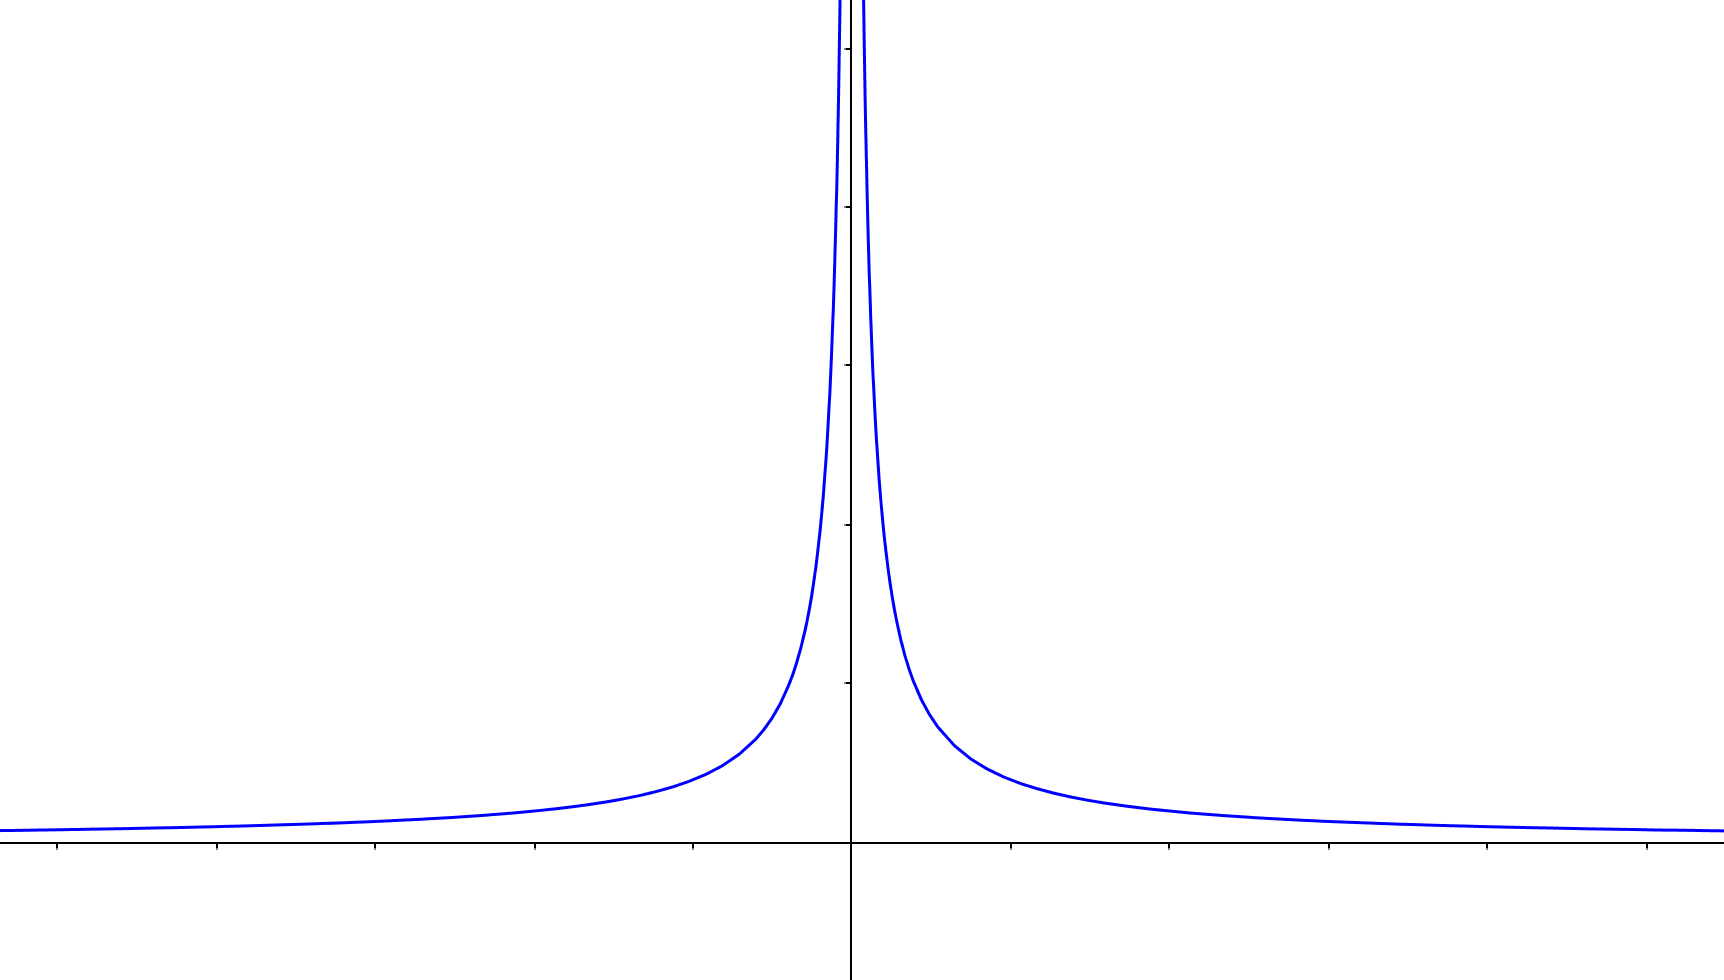
\includegraphics[scale=0.4]{allure}
\end{center}
\end{enumerate}

\begin{Exa}  Soit $\Sum{n \geq 1}{} u_n$ la s\'erie de fonctions d'une variable r\'eelle de terme g\'en\'eral $u_n$ d\'efini pour tout $n \in \N^*$ par : 
$$ \forall x \in \R ,\ u_n(x)=\dfrac{2x}{x^2+n^2\pi^2}$$
\begin{enumerate}
\item Montrer que $\Sum{n \geq 1}{} u_n$ converge simplement sur $\R$ tout entier.\\

\noindent On note $U=\dis \sum_{n=1}^{+\infty}{u_n}$ la somme de la s\'erie de fonctions $u_n$ .
\item Montrer que, pour tout $a > 0$ , $\Sum{n \geq 1}{} u_n$ converge normalement sur $[-a,a]$.
\item La s\'erie $\Sum{n \geq 1}{} u_n$ converge-t-elle normalement sur $\mathbb{R}$ ?
\item Montrer que $U$ est continue sur $\R$.
\end{enumerate}
\end{Exa}

\corr \begin{enumerate}
\item Pour tout réel $x$ et tout entier $n \geq 1$, on a :
$$\left| u_{n}\left( x\right) \right| \leq 
\frac{2\left| x\right| }{n^{2}\pi ^{2}}$$
Or la s\'{e}rie de terme g\'{e}n\'{e}ral $\dfrac{2\left| x\right| }{n^{2}\pi ^{2}}$ converge donc par critère de comparaison de séries à termes positifs, on en déduit que la série de terme général $u_{n}\left( x\right) $ converge absolument donc converge. Ainsi, $\Sum{n \geq 1}{} u_n$ converge simplement sur $\R$.
\item Si $x\in \left[ -a,a\right] $ alors pour tout $n \geq 1$, 
$$\left| u_{n}\left( x\right) \right| \leq \frac{2\left| x\right| }{n^{2}\pi ^{2}}\leq \frac{2\left|
a\right| }{n^{2}\pi ^{2}}$$
Ainsi $u_n$ est bornée sur $[-a,a]$ et on a :
$$ \Vert u_n \Vert_{[-a,a], \infty} \leq  \frac{2\left|a\right| }{n^{2}\pi ^{2}}$$
Or la s\'{e}rie de terme g\'{e}n\'{e}ral $\dfrac{2\left| a\right| }{n^{2}\pi ^{2}}$ converge (série de Riemann avec $2>1$) donc par critère de comparaison de séries à termes positifs, la série de fonctions de terme général $u_n$ converge normalement sur $[-a,a]$. Ainsi, pour tout $a > 0$ , $\Sum{n \geq 1}{} u_n$ converge normalement sur $[-a,a]$.
\item Pour tout $n \geq 1$, $u_n$ est impaire (évident), de classe $\mathcal{C}^1$ sur $\mathbb{R}$ et pour tout $x \in \mathbb{R}$,
$$u_n'(x) = 2 \times \frac{n^2\pi^2-x^2}{(x^2+n^2 \pi^2)^2}$$
En dressant le tableau de variations (suffisant sur $\mathbb{R}_+$ par imparité de la fonction), on en déduit que $u_n$ est bornée sur $\mathbb{R}$ et que l'on a :
$$ \Vert u_n \Vert_{\infty} = u_n( n \pi) = \frac{1}{n \pi}$$
Sachant que la série de terme général $\dfrac{1}{n\pi}$ diverge (série harmonique), on en déduit que la s\'{e}rie $\Sum{n \geq 1}{} u_{n}$ ne converge pas normalement sur $\mathbb{R}$.
\item Les fonctions $u_{n}$ ($n \geq 1$) sont continues sur $\mathbb{R}$ et on sait que la s\'{e}rie $\Sum{n \geq 1}{} u_{n}$ converge normalement et donc uniformément sur tout segment de $\mathbb{R}$ (car sur tout segment symétrique). Par théorème de continuité, on en déduit que $U$ est continue sur $\Bbb{R}$.
\end{enumerate}

\begin{Exa} Soit $S : x \mapsto \dis \sum_{n=0}^{+ \infty}  (-1)^n \dfrac{\cos^3(3^nx)}{3^n} \cdot$

\begin{enumerate}
\item Déterminer l'ensemble de définition, notée $I$, de $S$.
\item Donner une expression simple de $S(x)$ pour $x \in I$.
\end{enumerate}
\end{Exa}

\corr \begin{enumerate}
\item Posons pour tout $n \geq 0$, $f_n : x \mapsto (-1)^n \dfrac{\cos^3(3^nx)}{3^n} \cdot$

\medskip

\noindent Pour tout $n \geq 0$ et tout $x \in \mathbb{R}$, on a :
$$ \vert f_n(x) \vert \leq \frac{1}{3^n}$$
donc $f_n$ est bornée sur $\mathbb{R}$ et on a :
$$ 0 \leq \Vert f_n \Vert_{\infty} \leq \frac{1}{3^n}$$
La série de terme général $\dfrac{1}{3^n}$ converge (série géométrique avec une raison de module strictement inférieur à $1$) donc par critère de comparaison de séries à termes positifs, on en déduit que la série de fonctions de terme général $f_n$ converge normalement et donc en particulier simplement. Ainsi, $\dis S$ est définie sur $I = \mathbb{R}$.
\item Par linéarisation, on montre que pour tout $y \in \mathbb{R}$,
$$ \cos^3(y) = \frac{\cos(3y)+3\cos(y)}{4}$$.
Ainsi, pour tout $n \geq 1$ et tout $x \in \mathbb{R}$,
\begin{align*}
f_n(x)& = (-1)^n \dfrac{\cos^3(3^nx)}{3^n} \\
& = \frac{(-1)^n}{4} \times  \dfrac{cos(3^n(3x)+3\cos(3^nx))}{3^n}  \\
& = \frac{(-1)^n}{4} \times  \left(\dfrac{cos(3^{n+1} x)}{3^n}+\frac{\cos(3^nx))}{3^{n-1}} \right) \\
& = \frac{(-1)^n}{4} \times\dfrac{cos(3^{n+1} x)}{3^n}- \frac{(-1)^{n-1}}{4} \times\frac{\cos(3^nx))}{3^{n-1}} 
\end{align*}
Ainsi, pour tout $N \geq 1$, on a :
\begin{align*}
\sum_{n=0}^{N} f_n(x) & = f_0(x) + \sum_{n=1}^{N} \frac{(-1)^n}{4} \times\dfrac{cos(3^{n+1} x)}{3^n}- \frac{(-1)^{n-1}}{4} \times\frac{\cos(3^nx))}{3^{n-1}})  \\
& = \cos^3(x) + \frac{(-1)^N}{4} \times\dfrac{cos(3^{N+1} x)}{3^N} - \frac{1}{4} \cos(3x)     
\end{align*}
Or on a (par produit d'une suite bornée avec une suite convergente vers $0$) :
$$ \lim_{N \rightarrow + \infty} \frac{(-1)^N}{4} \dfrac{cos(3^{N+1} x)}{3^N} = 0$$
et ainsi :
$$ \sum_{n=0}^{+\infty} f_n(x)  = \cos^3(x) - \frac{1}{4} \cos(3x) = \frac{3}{4} \cos(x)$$
Finalement,
$$\dis \forall x \in I, \; S(x)= \dfrac{3}{4}\cos(x)$$
\end{enumerate}

\begin{Exa} Soit $(P_{n})_{n \geq 0}$ une suite de fonctions polynômiales de $\R$ dans $\R$. On suppose que cette suite converge uniformément vers une fonction $f$ sur $\R$. Montrer que la fonction $f$ est polynomiale.
\end{Exa}

\corr Soit $(P_{n})_{n \geq 0}$ une suite de fonctions polynômiales de $\R$ dans $\R$. On suppose que cette suite converge uniformément vers une fonction $f$ sur $\R$. Par définition, on a :
$$ \forall \varepsilon >0, \; \exists N \in \mathbb{N}, \; \forall n \geq N, \;  \forall x \in \mathbb{R}, \; \vert P_n(x)-f(x) \vert \leq \varepsilon$$
En particulier, pour $\varepsilon=1$, il existe un rang $N \in \mathbb{N}$, tel que pour tout $n \geq N$, $P_n-f$ est bornée sur $\mathbb{R}$ et tel que :
$$ \Vert P_n- f \Vert_{\infty} \leq 1$$
Ainsi, pour tout $n \geq N$,
$$ P_n-P_N = (P_n-f)-(P_N-f)$$
est une fonction polynômiale bornée sur $\mathbb{R}$ et donc constante. On a de plus pour tout $n \geq N$,
$$ P_n-P_N - (f-P_N) = f-P_N$$
donc $(P_n-P_N)$ converge uniformément vers $f-P_N$ sur $\mathbb{R}$ mais cette suite étant une suite de fonctions constantes, on en déduit qu'elle converge uniformément nécessairement vers une fonction constante $x \mapsto C$ où $C \in \mathbb{R}$. Par unicité de la limite, on a alors que :
$$ f-P_N=C$$
et donc $f=P_N+C$ est une fonction polynômiale.

\begin{Exa} Soit $(f_n)_{n \geq 1}$ la suite de fonctions définies pour tout $x \in \mathbb{R}_+$ par 
$$f_n(x) = \frac {nx}{1+n^2x^2}$$
\begin{enumerate}
\item Étudier la convergence simple de $(f_n)_{n \geq 1}$ sur $\mathbb{R}_+$.
\item Étudier la convergence uniforme de $(f_n)_{n \geq 1}$ sur $\mathbb{R}_+$ puis sur $[a, + \infty[$ pour $a>0$.
\end{enumerate}
\end{Exa}

\corr 

\begin{enumerate}
\item Soit $x \in \mathbb{R}_+$.

\begin{itemize}
\item Si $x=0$, alors pour tout $n \geq 1$, $f_n(0)=0$ et ainsi :
$$ \lim_{n \rightarrow + \infty} f_n(0)=0$$
\item Si $x \neq 0$ alors :
$$ f_n(x) \underset{n \rightarrow + \infty}{\sim} \dfrac{nx}{n^2x^2} = \dfrac{1}{nx}$$
Ainsi,
$$ \lim_{n \rightarrow + \infty} f_n(x) = 0$$
\end{itemize}
On en déduit que $(f_n)_{n \geq 1}$ converge simplement sur $\mathbb{R}_+$ vers la fonction nulle.
\item Proposons deux méthodes.

\medskip

\noindent $\rhd$ Supposons par l'absurde que $(f_n)_{n \geq 1}$ converge uniformément vers la fonction nulle sur $\mathbb{R}_+$. On en déduit qu'à partir d'un certain rang, $f_n$ est bornée et :
$$ \lim_{n \rightarrow + \infty} \Vert f_n \Vert_{\infty} = 0$$
Pour tout entier $n \geq 1$, $1/n \in \mathbb{R}_+$ donc à partir d'un certain rang :
$$ 0 \leq \left\vert f_n \left( \dfrac{1}{n} \right) \right\vert \leq \Vert f_n \Vert_{\infty}$$
Par théorème d'encadrement, on en déduit que :
$$ \lim_{n \rightarrow + \infty} f_n \left( \dfrac{1}{n} \right) = 0$$
Or pour tout entier $n \geq 1$,
$$ f_n \left( \dfrac{1}{n} \right) = \dfrac{1}{2}$$
C'est absurde. Ainsi, $(f_n)_{n \geq 1}$ ne converge pas uniformément vers la fonction nulle sur $\mathbb{R}_+$.

\medskip

\noindent $\rhd$ Soit $n \geq 1$. Étudions les variations de $f_n$. La fonction $f_n$ est dérivable sur $\mathbb{R}_+$ et pour tout $x \in \mathbb{R}_+$,
$$ f_n'(x) = n \times \dfrac{(1+n^2x^2)-x(2n^2x)}{(1+n^2x^2)^2} = n \times \dfrac{1-n^2x^2}{(1+n^2x^2)^2}$$
On en déduit que $f_n$ est croissante sur $[0,1/n]$ et décroissante sur $[1/n, + \infty[$. On a $f_n(0)=0$, $f_n(1/n)=1/2$ et 
$$ \lim_{x \rightarrow + \infty} f_n(x) = 0$$
Ainsi, $f_n$ est bornée sur $\mathbb{R}_+$ et 
$$ \Vert f_n \Vert_{\infty} = \dfrac{1}{2}$$
Ainsi, la suite de terme général $\Vert f_n \Vert_{\infty}$ tend pas vers $0$ quand $n$ tend vers $+ \infty$ donc $(f_n)_{n \geq 1}$ ne converge pas uniformément vers la fonction nulle sur $\mathbb{R}_+$.

\medskip

\noindent Soit $a>0$. D'après la méthode précédente, on sait que pour tout entier $n \geq 1$, $f_n$ est croissante sur $[0,1/n]$ et décroissante sur $[1/n, + \infty[$. On sait que $1/n$ tend vers $0$ quand $n$ tend vers $+ \infty$ donc à partir d'un certain rang, $1/n<a$ donc $f_n$ est décroissante sur $[a, + \infty[$ et avec la même méthode que précédemment on en déduit que :
$$  \Vert f_n \Vert_{\infty} = f_n(a)$$
Or $(f_n)_{n \geq 1}$ converge simplement vers la fonction nulle sur $\mathbb{R}_+$ et $a \in \mathbb{R}_+$ donc 
$$ \lim_{n \rightarrow + \infty} f_n(a) = 0$$
et ainsi, $(f_n)_{n \geq 1}$ converge uniformément vers la fonction nulle sur $[a, + \infty[$.

\end{enumerate}

\begin{Exa} Montrer que la limite simple d'une suite de fonctions croissantes de $I$ vers $\mathbb{R}$ est croissante.
\end{Exa}

\corr Soit $(f_n)_{n \geq 0}$, une suite de fonctions croissantes de $I$ dans $\mathbb{R}$, convergeant simplement vers $f : I \rightarrow \mathbb{R}$. Montrons que $f$ est croissante sur $I$. Soit $(x,y) \in I^2$ tel que $x \leq y$. Pour tout entier $n \geq 0$, $f_n$ est croissante sur $I$ donc $f_n(x) \leq f_n(y)$. Par passage à la limite pour des inégalités larges, on en déduit que $f(x) \leq f(y)$. Ainsi, $f$ est croissante sur $I$.


\begin{Exa} Étudier la convergence simple, normale puis uniforme de $\dis \sum f_n$ sur $\mathbb{R}_+$ où pour tout entier $n \geq 0$ et tout $x \in \mathbb{R}_+$, $f_n(x) = nx^2e^{-x\sqrt{n}}.$
\end{Exa} 

\corr 

\noindent $\rhd$ Étudions la convergence simple. Soit $x \in \mathbb{R}_+$.

\begin{itemize}
\item Si $x=0$ alors pour tout entier $n \geq 0$, $f_n(0)=0$ et la série de terme général $f_n(0)$ est donc convergente.
\item Si $x \neq 0$ alors :
$$ f_n(x) \underset{n \rightarrow + \infty}{=} o \left( \dfrac{1}{n^2} \right)$$
car 
$$ n^2f_n(x) = n^3x^2e^{-x\sqrt{n}} \underset{n \rightarrow + \infty}{\longrightarrow} 0$$
par théorème des croissances comparées. La série de terme général $1/n^2$ converge (série de Riemann avec $2>1$) donc par critère de comparaison, on en déduit que la série de terme général $f_n(x)$ converge absolument donc converge.
\end{itemize}
Ainsi, $\dis \sum f_n$ converge simplement sur $\mathbb{R}_+$.

\medskip

\noindent $\rhd$ Supposons par l'absurde que $\dis \sum f_n$ converge normalement sur $\mathbb{R}_+$. Pour tout entier $n \geq 0$, $f_n$ est bornée sur $\mathbb{R}_+$ et :
$$ 0 \leq \vert f_n(1/\sqrt{n}) \vert \leq \Vert f_n \Vert_{\infty}$$
Par critère de comparaison des séries à termes positifs, on en déduit que la série de terme général $f_n(1/\sqrt{n})$ converge absolument donc converge. Or pour tout entier $n \geq 1$,
 $$ f_n(1/\sqrt{n}) = e^{-1}$$
Cette série diverge grossièrement : c'est absurde. Ainsi, $\dis \sum f_n$ ne converge pas normalement sur $\mathbb{R}_+$.

\medskip

\noindent $\rhd$ Posons pour tout $x \in \mathbb{R}_+$ et tout entier $n \geq 0$,
$$ R_n(x) = \sum_{k=n+1}^{+ \infty} f_k(x)$$
Par positivité des termes, on a :
$$ \vert R_n(x) \vert = R_n(x) \geq f_{n+1}(x)$$
La fonction $f_{n+1}$ est dérivable sur $\mathbb{R}_+$ et pour tout réel $x \geq 0$,
$$ f_{n+1}'(x) = (n+1)x (2-x \sqrt{n+1})e^{-x \sqrt{n+1}}$$
Ainsi, la fonction $f_{n+1}$ est positive sur $\mathbb{R}_+$, croissante sur $[0, 2/ \sqrt{n+1}]$ et décroissante sur $[2/\sqrt{n+1}, + \infty[$. On en déduit que $f_{n+1}$ est bornée sur $\mathbb{R}_+$ et :
$$ \Vert f_{n+1} \Vert_{\infty} = f_{n+1}(2/\sqrt{n+1}) = 4 e^{-2}$$
Supposons par l'absurde la série étudiée converge uniformément sur $\mathbb{R}_+$. Alors la suite des restes converge uniformément vers $0$ : à partir d'un certain rang, $R_n$ est bornée et :
$$ \lim_{n \rightarrow + \infty} \Vert R_n \Vert_{ \infty} = 0$$
Or pour tout $x \in \mathbb{R}_+$,
$$  \vert R_n(x) \vert \geq f_{n+1}(x)$$
donc 
$$ \Vert R_n \Vert_{\infty} \geq \Vert f_{n+1} \Vert_{\infty} = 4 e^{-1}$$
C'est absurde ! Ainsi, la série étudiée ne converge pas uniformément sur $\mathbb{R}_+$.

\begin{Exa} Soient $\alpha \in \R$ et $(f_n)_{n \geq 1}$ la suite de fonctions définies pour tout $x \in [0,1]$ par 
$$f_n(x) = n^\alpha x(1-x)^n$$

\begin{enumerate}
 \item Étudier la convergence simple de $(f_n)_{n \geq 1}$.
 \item Y a-t-il convergence uniforme ?
  \end{enumerate}
\end{Exa}

\corr 

\begin{enumerate}
\item Remarquons que pour tout entier $n \geq 1$,
$$ f_n(0)=f_n(1)=0$$
Ainsi,
$$ \lim_{n \rightarrow + \infty} f_n(0) = \lim_{n \rightarrow + \infty} f_n(1) = 0$$
Soit $x \in ]0,1[$. Pour tout entier $n \geq 1$,
$$ f_n(x) = n^{\alpha} x e^{n \ln(1-x)}$$
Sachant que $\ln(1-x)$ est négatif, on en déduit que :
$$ \lim_{n \rightarrow + \infty}e^{n \ln(1-x)} = 0$$
Par produit de limite (et par théorème des croissances comparées si $\alpha>0$, on en déduit que :
$$ \lim_{n \rightarrow + \infty} f_n(x) = 0$$
Ainsi, $(f_n)_{n \geq 1}$ converge simplement vers la fonction nulle sur $[0,1]$.
\item Pour tout entier $n \geq 1$, $f_n$ est dérivable sur $[0,1]$ et pour tout $x \in [0,1]$,
$$ f_n'(x) = n^{\alpha} ((1-x)^n + x (-1) n (1-x)^{n-1}) = n^{\alpha} (1-x)^{n-1} (1-x-nx) = n^{\alpha} (1-x)^{n-1} (1-(n+1)x)$$
Ainsi, $f_n$ est croissante sur $[0, 1/(n+1)]$, décroissante sur $[1/(n+1), 1]$. De plus,
$$ f_n(0)=0, \; f_n(1)=0 \; \hbox{ et } f_n(1/(n+1)) =n^{\alpha} \times \dfrac{1}{n+1} \left(1- \dfrac{1}{n+1}\right)^{n}$$
On en déduit que $f_n$ est bornée sur $[0,1]$ et :
$$ \Vert f_n \Vert_{\infty} =   \dfrac{n^{\alpha}}{n+1} \left(1- \dfrac{1}{n+1}\right)^{n}$$
On sait que :
$$\left(1- \dfrac{1}{n+1}\right)^{n} = \exp \left(n \left(1- \dfrac{1}{n+1}\right) \right) $$
Or quand $n$ tend vers $+ \infty$,
$$ \ln \left(1- \dfrac{1}{n+1}\right) \underset{+ \infty}{\sim} - \dfrac{1}{n+1}$$
donc 
$$ n \ln \left(1- \dfrac{1}{n+1}\right) \underset{+ \infty}{\sim} - \dfrac{n}{n+1} \underset{+ \infty}{\sim} -1$$
Par continuité de l'exponentielle en $-1$, on en déduit que :
$$ \lim_{n \rightarrow + \infty} \left(1- \dfrac{1}{n+1}\right)^{n} = e^{-1}$$
Ainsi,
$$  \Vert f_n \Vert_{\infty} \underset{+ \infty}{\sim} \dfrac{n^{\alpha}}{n+1} e^{-1} \underset{+ \infty}{\sim} n^{\alpha-1} e^{-1}$$
On en déduit que $\Vert f_n \Vert_{\infty}$ tend vers $0$ quand $n$ tend vers $+ \infty$ si et seulement si $\alpha<1$ donc $(f_n)_{n \geq 1}$ converge uniformément vers la fonction nulle sur $[0,1]$ si et seulement si $\alpha<1$.
\end{enumerate}

\begin{Exa} Pour tout entier $n \geq 0$, on note $f_n$ la fonction définie sur $\mathbb{R}_+$ par :
$$ f_n(x) = \frac{x^n e^{-x}}{n!}$$

\begin{enumerate}
\item Déterminer la limite simple de $(f_n)_{n \geq 0}$ sur $\mathbb{R}_+$.
\item Montrer qu'il y a convergence uniforme (on pourra utiliser la formule de Stirling).
\end{enumerate}
\end{Exa} 

\corr 

\begin{enumerate}
\item Soit $x \in \mathbb{R}_+$. La série de terme général $\dfrac{x^n}{n!}$ converge (série exponentielle) donc :
$$ \lim_{n \rightarrow + \infty}  \frac{x^n}{n!} = 0$$
donc 
$$ \lim_{n \rightarrow + \infty} f_n(x)=0$$
Ainsi, $(f_n)_{n \geq 0}$ converge simplement vers la fonction nulle sur $\mathbb{R}_+$.
\item Pour tout entier $n \geq 0$, $f_n$ est dérivable sur $\mathbb{R}_+$ et pour tout $x \in \mathbb{R}_+$,
$$ f_n'(x) = \dfrac{1}{n!} (nx^{n-1} e^{-x} + x^n (-e^{-x})) = \dfrac{1}{n!} x^{n-1} e^{-x} (n-x)$$
Ainsi, $f_n$ est croissante sur $[0,n]$ et décroissante sur $[n,+ \infty[$. On a :
$$ f_n(0)=0, \; f_n(n) = \dfrac{n^n e^{-n}}{n!} \; \hbox{ et } \lim_{x \rightarrow + \infty} f_n(x) = 0$$
par théorème des croissances comparées si $n>0$. On en déduit que $f_n$ est bornée sur $\mathbb{R}_+$ et 
$$ \Vert f_n \Vert_{\infty} = \dfrac{n^n e^{-n}}{n!}$$
D'après la formule de Stirling, on a :
\begin{align*}
 \Vert f_n \Vert_{\infty} & \underset{+ \infty}{\sim} \dfrac{n^n e^{-n}}{(n/e)^n \sqrt{2 \pi n}} \\
 & \underset{+ \infty}{\sim} \dfrac{1}{\sqrt{2 \pi n}} 
\end{align*}
Ainsi,
$$ \lim_{n \rightarrow + \infty} \Vert f_n \Vert_{\infty} = 0$$
On en déduit que $(f_n)_{n \geq 1}$ converge uniformément vers la fonction nulle sur $\mathbb{R}_+$.
\end{enumerate}

\begin{Exa} Pour $n\in\N^*,$ on considère la fonction $f_n : \, ] 1,+\infty[ \rightarrow \mathbb{R}$ définie par :
$$ f_n(x)=\frac{(-1)^n}{\ln(nx)}$$

\begin{enumerate}
	\item Justifier que $F : x\longmapsto \dis\sum_{n=1}^{+\infty} f_n(x)$ est bien définie sur $]1,+\infty[.$
	
	\item Démontrer que $\dis\sum f_n$ converge uniformément sur $]1,+\infty[.$ 
	
	\item Montrer que $F$ est continue sur $]1,+\infty[$ et déterminer $\dis\lim_{x \rightarrow 1}F(x)$ et  $\dis\lim_{x \rightarrow  +\infty}F(x)$.
	
	\item Démontrer que $F$ est de classe ${\cal C}^1$ sur $]1,+\infty[$ et préciser les variations $F.$
\end{enumerate}
\end{Exa}

\corr  

\begin{enumerate}
\item Pour tout entier $n \geq 1$ et tout réel $x>1$, $nx>1$ donc $(\ln(nx))_{n \geq 1}$ est une suite strictement positive. De plus, elle est strictement croissante (par croissance du logarithme). On en déduit que la suite de terme général $1/\ln(nx)$ est strictement positive et décroissante. De plus,
$$ \lim_{n \rightarrow + \infty} \dfrac{1}{\ln(nx)} = 0$$
D'après le critère spécial des séries alternées, on en déduit que la série de terme général 
$$ f_n(x)  =\frac{(-1)^n}{\ln(nx)}$$
converge. Ainsi, $F$ est bien définie sur $]1, + \infty[$.
\item Soit $x \in ]1, + \infty[$. Notons pour tout entier $n \geq 1$,
$$ R_n(x) = \sum_{k=n+1}^{+ \infty} f_k(x)$$
D'après le critère spécial des séries alternées (hypothèses vérifiées dans la question précédente), on a :
$$ \vert R_n(x) \vert \leq \vert f_{n+1}(x) \vert  = \dfrac{1}{\ln((n+1)x)} \leq \dfrac{1}{\ln(n+1)}$$
car $x>1$. Ainsi, $R_n$ est bornée sur $]1, + \infty[$ et :
$$ 0 \leq \Vert R_n \Vert_{\infty} \leq \dfrac{1}{\ln(n+1)}$$
Par théorème d'encadrement, on en déduit que la suite (des restes) de terme général $ \Vert R_n \Vert_{\infty}$ converge vers $0$. Ainsi, $\dis\sum f_n$ converge uniformément sur $]1,+\infty[.$ 
\item 

\noindent $\rhd$ Pour tout entier $n \geq 1$, $f_n$ est continue et sur $]1, + \infty[$ et $\dis\sum f_n$ converge uniformément sur $]1,+\infty[.$ Par théorème de continuité, on en déduit que $F= \sum_{n=1}^{+ \infty} f_n$ est continue sur $]1, + \infty[$.

\medskip

\noindent $\rhd$ Déterminons par une première méthode la limite de $F$ en $+ \infty$. D'après le critère spécial des séries alternés (hypothèses vérifiées dans la question $1$), on sait que pour tout $x>1$,
$$ 0 \leq \left\vert \sum_{n=1}^{+ \infty} \dfrac{(-1)^n}{\ln(nx)} \right\vert \leq \left\vert \dfrac{(-1)^1}{\ln(x)} \right\vert = \dfrac{1}{\ln(x)}$$
Par théorème d'encadrement, on en déduit que :
$$ \lim_{x \rightarrow + \infty} \sum_{n=1}^{+ \infty} \dfrac{(-1)^n}{\ln(nx)} = 0$$
et ainsi
$$ \lim_{x \rightarrow + \infty} F(x)= 0$$

\medskip

\noindent $\rhd$ Déterminons par une deuxième méthode la limite de $F$ en $+ \infty$.

\begin{itemize}
\item $\dis\sum f_n$ converge uniformément sur $]1,+\infty[$ (dont $+ \infty$ est une extrémité).
\item Pour tout entier $n \geq 1$,
$$ \lim_{x \rightarrow + \infty} f_n(x) = 0$$
par produit d'un terme bornée et d'une fonction ayant pour limite $0$.
\end{itemize}
Par théorème d'interversion limite/somme, on en déduit que $F$ a une limite en $+ \infty$ et :
$$ \lim_{x \rightarrow + \infty}  F(x) = \lim_{x \rightarrow + \infty} \sum_{n=1}^{+ \infty} f_n(x) =  \sum_{n=1}^{+ \infty} \lim_{x \rightarrow + \infty} f_n(x)=   \sum_{n=1}^{+ \infty}  0 = 0$$

\medskip

\noindent $\rhd$ Pour tout $x \in ]1, + \infty[$,
$$ F(x) = - \dfrac{1}{\ln(x)} + \sum_{n=2}^{+ \infty} f_n(x)$$
La série $\sum_{n \geq 2} f_n$ converge uniformément sur $]1, + \infty[$ donc $1$ est une extrémité. Pour tout $n \geq 2$,
$$ \lim_{x \rightarrow 1} f_n(x) = \dfrac{(-1)^n}{\ln(n)}$$
Par théorème d'interversion limite/somme, on en déduit que la somme de $\sum_{n \geq 2} f_n$ admet une limite finie en $1^+$ valant :
$$ \sum_{n=2}^{+ \infty} \dfrac{(-1)^n}{\ln(n)}$$
Ainsi, $x \mapsto F(x) + \dfrac{1}{\ln(x)}$ admet une limite finie quand $x$ tend vers $1^+$. Or :
$$ \lim_{x \rightarrow 1^+} \dfrac{1}{\ln(x)} = + \infty$$
On en déduit que $F$ admet pour limite $- \infty$ en $1^{+}$ (par somme d'une fonction ayant cette limite et d'une fonction admettant une limite finie).
\item Vérifions les hypothèses du théorème de dérivation d'une somme de série de fonctions.
\begin{itemize}
\item La série de fonctions $\dis \sum f_n$ converge simplement sur $]1, + \infty[$.
\item Pour tout entier $n \geq 1$, $f_n$ est de classe $\mathcal{C}^1$ sur $]1, + \infty[$ et pour tout réel $x>1$,
$$ f_n'(x) = (1)^n \dfrac{-1/x}{\ln(nx)^2} = \dfrac{(-1))^{n+1}}{x \ln(nx)^2}$$
Soit $x>1$. La suite de terme général $\ln(nx)$ est croissante et strictement positive donc la suite de terme général $\ln(nx)^2$ est croissante et ainsi la suite de terme général 
$$ \vert f_n'(x) \vert = \dfrac{1}{x \ln(nx)^2}$$
est décroissante et positive. De plus,
$$ \lim_{n \rightarrow + \infty} \vert f_n'(x) \vert = 0$$
Ainsi, la série de terme général $f_n'(x)$ est une série alternée et les hypothèses du critère spécial sont vérifiées. Ainsi, la série de terme général $f_n'(x)$ est converge. Posons pour tout entier $n \geq 1$ et $x \in ]1, + \infty[$,
$$ R_n(x) = \sum_{k=n+1}^{+ \infty} f_k'(x)$$
D'après le critère spécial :
$$ \vert R_n(x) \vert \leq \vert f_{n+1}'(x) \vert = \dfrac{1}{x \ln((n+1)x)^2} \leq \dfrac{1}{\ln(n+1)^2}$$
car $x>1$. Ainsi, $R_n$ est bornée sur $]1, + \infty[$ et :
$$ 0 \leq \Vert R_n \Vert_{\infty} \leq \dfrac{1}{\ln(n+1)^2}$$
Par théorème d'encadrement, on en déduit que la suite de terme général $\Vert R_n \Vert_{\infty}$ converge et :
$$ \lim_{n \rightarrow + \infty} \Vert R_n \Vert_{\infty} = 0$$
Ainsi, $\dis \sum f_n'$ converge uniformément sur $]1, + \infty[$.
\end{itemize}
Par théorème de dérivation d'une somme de séries de fonctions, on en déduit que $F$ est de classe $\mathcal{C}^1$ sur $]1, + \infty[$ et pour tout réel $x>1$,
$$ F'(x) = \sum_{k=1}^{+ \infty} \dfrac{(-1))^{k+1}}{x \ln(kx)^2}$$
D'après le critère spécial, $F'(x)$ est du signe de :
$$ \dfrac{(-1))^{2}}{x \ln(x)^2} = \dfrac{1}{x \ln(x)^2}>0$$
Ainsi, $F$ est croissante sur $]1, + \infty[$.


\end{enumerate}

\begin{Exa} Pour tout entier $n \geq 1$, on note $f_n$ la fonction définie sur $\mathbb{R}_+$ par 
$$ f_n(x) = \frac{x}{n+x}$$
Étudier la convergence uniforme de $(f_n)_{n \geq 1}$ sur $\mathbb{R}_+$ puis sur un segment de $\mathbb{R}_+$.
\end{Exa}

\corr 

\noindent $\rhd$ Pour tout $x \in \mathbb{R}_+$,
$$ \lim_{n \rightarrow + \infty} f_n(x) = 0$$
Ainsi, $(f_n)_{n \geq 1}$ converge simplement vers la fonction nulle sur $\mathbb{R}_+$.

\medskip

\noindent $\rhd$ Supposons par l'absurde que $(f_n)_{n \geq 1}$ converge uniformément vers la fonction nulle sur $\mathbb{R}_+$. A partir d'un certain rang, $f_n$ est bornée et on a pour tout entier $n \geq 1$,
$$ 0 \leq \vert f_n(n) \vert \leq \Vert f_n \Vert_{\infty}$$
Par théorème d'encadrement, on en déduit que :
$$ \lim_{n \rightarrow + \infty} f_n(n) = 0$$
C'est absurde car pour tout entier $n \geq 1$,
$$ f_n(n) = \dfrac{n}{2n} = \dfrac{1}{2}$$
Ainsi,  $(f_n)_{n \geq 1}$ ne converge pas uniformément vers la fonction nulle sur $\mathbb{R}_+$.

\medskip

\noindent $\rhd$ Soit $(a,b) \in \mathbb{R}_+^2$ tel que $a <b$. Pour tout entier $n \geq 1$ et $x \in [a,b]$, $n+x \geq n+a>0$ donc par décroissance de la fonction inverse :
$$ 0 \leq \dfrac{1}{n+x} \leq \dfrac{1}{n+a}$$
De plus, $0 \leq x \leq b$ donc 
$$ 0 \leq \dfrac{x}{n+x} \leq \dfrac{b}{n+a}$$
Ainsi, $f_n$ est bornée sur $[a,b]$ et :
$$ 0 \leq \Vert f_n \Vert_{[a,b],\infty} \leq \dfrac{b}{n+a}$$
On a :
$$ \lim_{n \rightarrow + \infty}  \dfrac{b}{n+a} = 0$$
Par théorème d'encadrement, on en déduit que la suite de terme général $\Vert f_n \Vert_{[a,b],\infty}$ converge et :
$$ \lim_{n \rightarrow + \infty} \Vert f_n \Vert_{[a,b],\infty} = 0$$
Ainsi, $(f_n)_{n \geq 1}$ converge uniformément vers la fonction nulle sur $[a,b]$.

\begin{Exa} Étudier la convergence simple, normale et uniforme de $\dis \sum f_n$ sur $\mathbb{R}_+^*$ où pour tout entier $n \geq 0$ et tout $x \in \mathbb{R}_+^*$, 
$$ f_n(x) = \frac{1}{n+n^3x^2}$$
Cette série converge t-elle uniformément sur tout segment de $\mathbb{R}_+^*$ ?
\end{Exa} 

\corr 

\noindent $\rhd$ Soit $x \in \mathbb{R}_+^*$. La série de terme général $f_n(x)$ est à termes positifs et :
$$ f_n(x) \underset{+ \infty}{\sim} \dfrac{1}{n^3x^2}$$
La série de terme général positif $1/n^3$ converge (série de Riemann avec $3>1$). Par critère de comparaison des séries à termes positifs, on en déduit que la série de terme général $f_n(x)$ converge. Ainsi, $\dis \sum f_n$ converge simplement sur $\mathbb{R}_+^*$.

\medskip

\noindent $\rhd$ Supposons par l'absurde que $\dis \sum f_n$ converge uniformément sur $\mathbb{R}_+^*$. Pour tout entier $n \geq 1$,
$$ \lim_{x \rightarrow 0} f_n(x) = \dfrac{1}{n}$$
Or $0$ est une extrémité de $\mathbb{R}_+^*$ donc par théorème d'interversion limite-somme, on en déduit que la série de terme général $1/n$ diverge ce qui est absurde. Ainsi, $\dis \sum f_n$ ne converge pas uniformément sur $\mathbb{R}_+^*$ et donc ne converge pas normalement sur $\mathbb{R}_+^*$.

\medskip

\noindent $\rhd$ Soit $(a,b) \in \mathbb{R}_+^*$ tel que $a<b$. Pour tout entier $n \geq 1$ et tout $x \in [a,b]$, $n+n^3x^2 \geq n+n^3a^2 >0$. Par décroissance de la fonction inverse sur $\mathbb{R}_+^*$,
$$ 0 \leq f_n(x) \leq \dfrac{1}{n+n^3a^2} = f_n(a)$$
Ainsi $f_n$ est bornée sur $[a,b]$ et on a :
$$ 0 \leq \Vert f_n \Vert_{\infty} \leq f_n(a)$$
La série de terme général $f_n(a)$ converge (la série de fonctions converge simplement sur $\mathbb{R}_+^*$) donc par critère de comparaison des séries à termes positifs, on en déduit que $\dis \sum f_n$ converge normalement sur $[a,b]$ et donc converge uniformément sur $[a,b]$.

\begin{Exa} Donner l'ensemble de définition et de continuité de la fonction $f$ définie par 
  \[
  f(x) = \sum_{n = 0}^{ + \infty} \e^{ - x\sqrt n}
  \]
 Déterminer la limite en $ + \infty$ de $f$.
 \end{Exa}
 
 
\corr 

\noindent $\rhd$ Soit $x \in \mathbb{R}$.
\begin{itemize}
\item Si $x<0$ alors $-x>0$ donc :
$$ \lim_{n \rightarrow + \infty} \e^{ - x\sqrt n} = + \infty$$
La série de terme général $\e^{ - x\sqrt n}$ diverge donc grossièrement.
\item Si $x=0$ alors pour tout entier $n \geq 0$, $\e^{ - x\sqrt n}=1$ donc la série de terme général $\e^{ - x\sqrt n}$ diverge donc grossièrement.
\item Si $x>0$ alors par théorème des croissances comparées,
$$ \e^{ - x\sqrt n} = \underset{n \rightarrow + \infty}{=} o \left( \dfrac{1}{n^2} \right)$$
La série de terme général $1/n^2$ converge (série de Riemann avec $2>1$). Par critère de comparaison, on en déduit que la série de terme général $ \e^{ - x\sqrt n} $ converge absolument donc converge.
\end{itemize}
Ainsi, $f$ est définie sur $\mathbb{R}_+^*$.

\medskip

\noindent Notons pour tout entier $n \geq 0$, $f_n$ la fonction définie sur $\mathbb{R}_+^*$ par 
$$f_n(x)= \e^{ - x\sqrt n}$$
Soit $a \in \mathbb{R}_+^*$. Pour tout entier $n \geq 0$, la fonction $f_n$ est décroissante sur $\mathbb{R}_+$ donc :
$$ 0 \leq f_n(x) \leq f_n(a)$$
Ainsi, $f_n$ est bornée sur $[a, + \infty[$ et :
$$ 0 \leq \Vert f_n \Vert_{[a, + \infty[, \infty} \leq f_n(a)$$
La série de terme général $f_n(a)$ converge (la série de fonctions converge simplement sur $\mathbb{R}_+^*$) donc par critère de comparaison, on en déduit que $\dis \sum f_n$ converge normalement et donc uniformément sur $[a, + \infty[$. Par théorème de continuité d'une somme de série de fonctions, on en déduit que $f$ est continue sur $[a, + \infty[$ pour tout $a>0$ donc elle continue sur $\mathbb{R}_+^*$.

\medskip

\noindent $\rhd$ On a :
$$ \lim_{x \rightarrow + \infty} f_0(x) = \lim_{x \rightarrow + \infty} 1 = 1$$
et pour tout entier $n \geq 1$,
$$ \lim_{x \rightarrow + \infty} f_n(x) = 0$$
La série $\dis \sum f_n$ converge uniformément sur $[1, + \infty[$ dont $+ \infty$ est une extrémité. Par théorème d'interversion limite-somme, on en déduit que $f$ admet une limite en $+ \infty$ et on a :
$$ \lim_{x \rightarrow + \infty} f(x) = \sum_{n=0}^{+ \infty} \lim_{x \rightarrow + \infty} f_n(x) = 1$$

\begin{Exa} Posons :
$$f: x \mapsto \sum_{n=1}^{+ \infty} \dfrac{1}{n^2+x^2}$$
Montrer que $f$ est définie et de classe $\mathcal{C}^{\infty}$ sur $\mathbb{R}$.
\end{Exa} 

\corr On pose pour tout entier $n \geq 1$ et tout $x \in \mathbb{R}$,
$$ f_n(x) = \dfrac{1}{n^2+x^2}$$

\medskip

\noindent $\rhd$ Pour tout $x \in \mathbb{R}$ et tout entier $n \geq 1$, $n^2+x^2 \geq n^2>0$ donc par décroissance de la fonction inverse sur $\mathbb{R}$ :
$$ 0 \leq f_n(x) \leq \dfrac{1}{n^2}$$
Ainsi, $f_n$ est bornée sur $\mathbb{R}$ et on a :
$$ 0 \leq \Vert f_n \Vert_{\infty} \leq \dfrac{1}{n^2}$$
La série de terme général $1/n^2$ converge (série de Riemann avec $2>1$). Par critère de comparaison, on en déduit que $\dis \sum f_n$ converge normalement sur $\mathbb{R}$. Ainsi, pour tout réel $x$, la série de terme général $f_n(x)$ converge et $f$ est donc bien définie sur $\mathbb{R}$.

\medskip

\noindent $\rhd$ Pour tout entier $n \geq 1$ et tout $x \in \mathbb{R}$,
\begin{align*}
f_n(x) & = \dfrac{1}{x^2+n^2} \\
& = \dfrac{1}{(x-in)(x+in)} \\
& = \dfrac{1}{2in} \times \dfrac{(x+in)-(x-in)}{(x-in)(x+in)} \\
& = \dfrac{1}{2in} \times \left( \dfrac{1}{x-in} - \dfrac{1}{x+in} \right)
\end{align*}
La fonction $f_n$ est de classe $\mathcal{C}^{\infty}$ sur $\mathbb{R}$ et on montre par récurrence (après conjecture) que pour tout entier $k \geq 0$ :
$$ \forall x \in \mathbb{R}, \; f_n^{(k)}(x) = \dfrac{(-1)^k k!}{2in} \left( \dfrac{1}{(x-in)^{k+1}} - \dfrac{1}{(x+in)^{k+1}} \right) $$
Sachant que $x$ est réel et $in$ est imaginaire pur, on a :
$$ \vert x-in \vert = \vert x+in \vert$$
Ainsi, d'après l'inégalité triangulaire, on en déduit que pour tout $(n,k) \in \mathbb{N}^* \times \mathbb{N}$ et tout $x \in \mathbb{R}$,
\begin{align*}
\vert  f_n^{(k)}(x) \vert & \leq \dfrac{k!}{2n} \times \dfrac{2}{\vert x-in \vert^{k+1}} \\
& = \dfrac{k!}{n} \times \dfrac{1}{(x^2+n^2)^{(k+1)/2}} \\
& \leq \dfrac{k!}{n^{k+2}}  
\end{align*}
car $x^2+n^2 \geq n^2$. On en déduit que $f_n^{(k)}$ est bornée sur $\mathbb{R}$ et on a :
$$ 0 \leq \Vert f_n^{(k)} \Vert_{\infty} \leq \dfrac{k!}{n^{k+2}} $$
La série de terme général $dfrac{1}{n^{k+2}}$ converge car $k+2 \geq 2$ (série de Riemann convergente) donc par critère de comparaison on en déduit que $\dis \sum_{n \geq 1} f_n^{(k)}$ converge normalement sur $\mathbb{R}$.

\medskip

\noindent Par théorème de dérivation, on en déduit que $f$ est de classe $\mathcal{C}^k$ sur $\mathbb{R}$ pour tout entier $k \geq 0$. Ainsi, $f$ est de classe $\mathcal{C}^{\infty}$ sur $\mathbb{R}$.
\end{document}